\chapter{Tree}

\section{Binary Search Tree}
The search binary tree data structure is capable of suporting both \textit{dictionary} and \textit{priority queue} operation in time proportional to the height of the tree.
Note that in the average case, for randomly constructed tree , the hight is $\Theta(log n)$ but the worst case is bad, since there is always a way to arrange it items s.t. it degrade to a linked list, with height $O(n)$. Self balancing trees ensure that the hight is always logaritmic in the number of nodes (red-black, or AVL tree are two names for such trees).

Let's start stating what is the invariant that makes the binary search tree so powerful. The binary search property always hold for each node of the tree, and all the operations always manintain such property.


\textbf{For each node of the three $x$ then all the nodes in the left subtree rooted at $x.left$ are strictly smaller  then $x.key$ and all the nodes in the right subtree rooted at $x.right$ are greater or equal than $x.key$.
}

	\begin{figure}
	\label{fig:tree_visits}
	\centering
		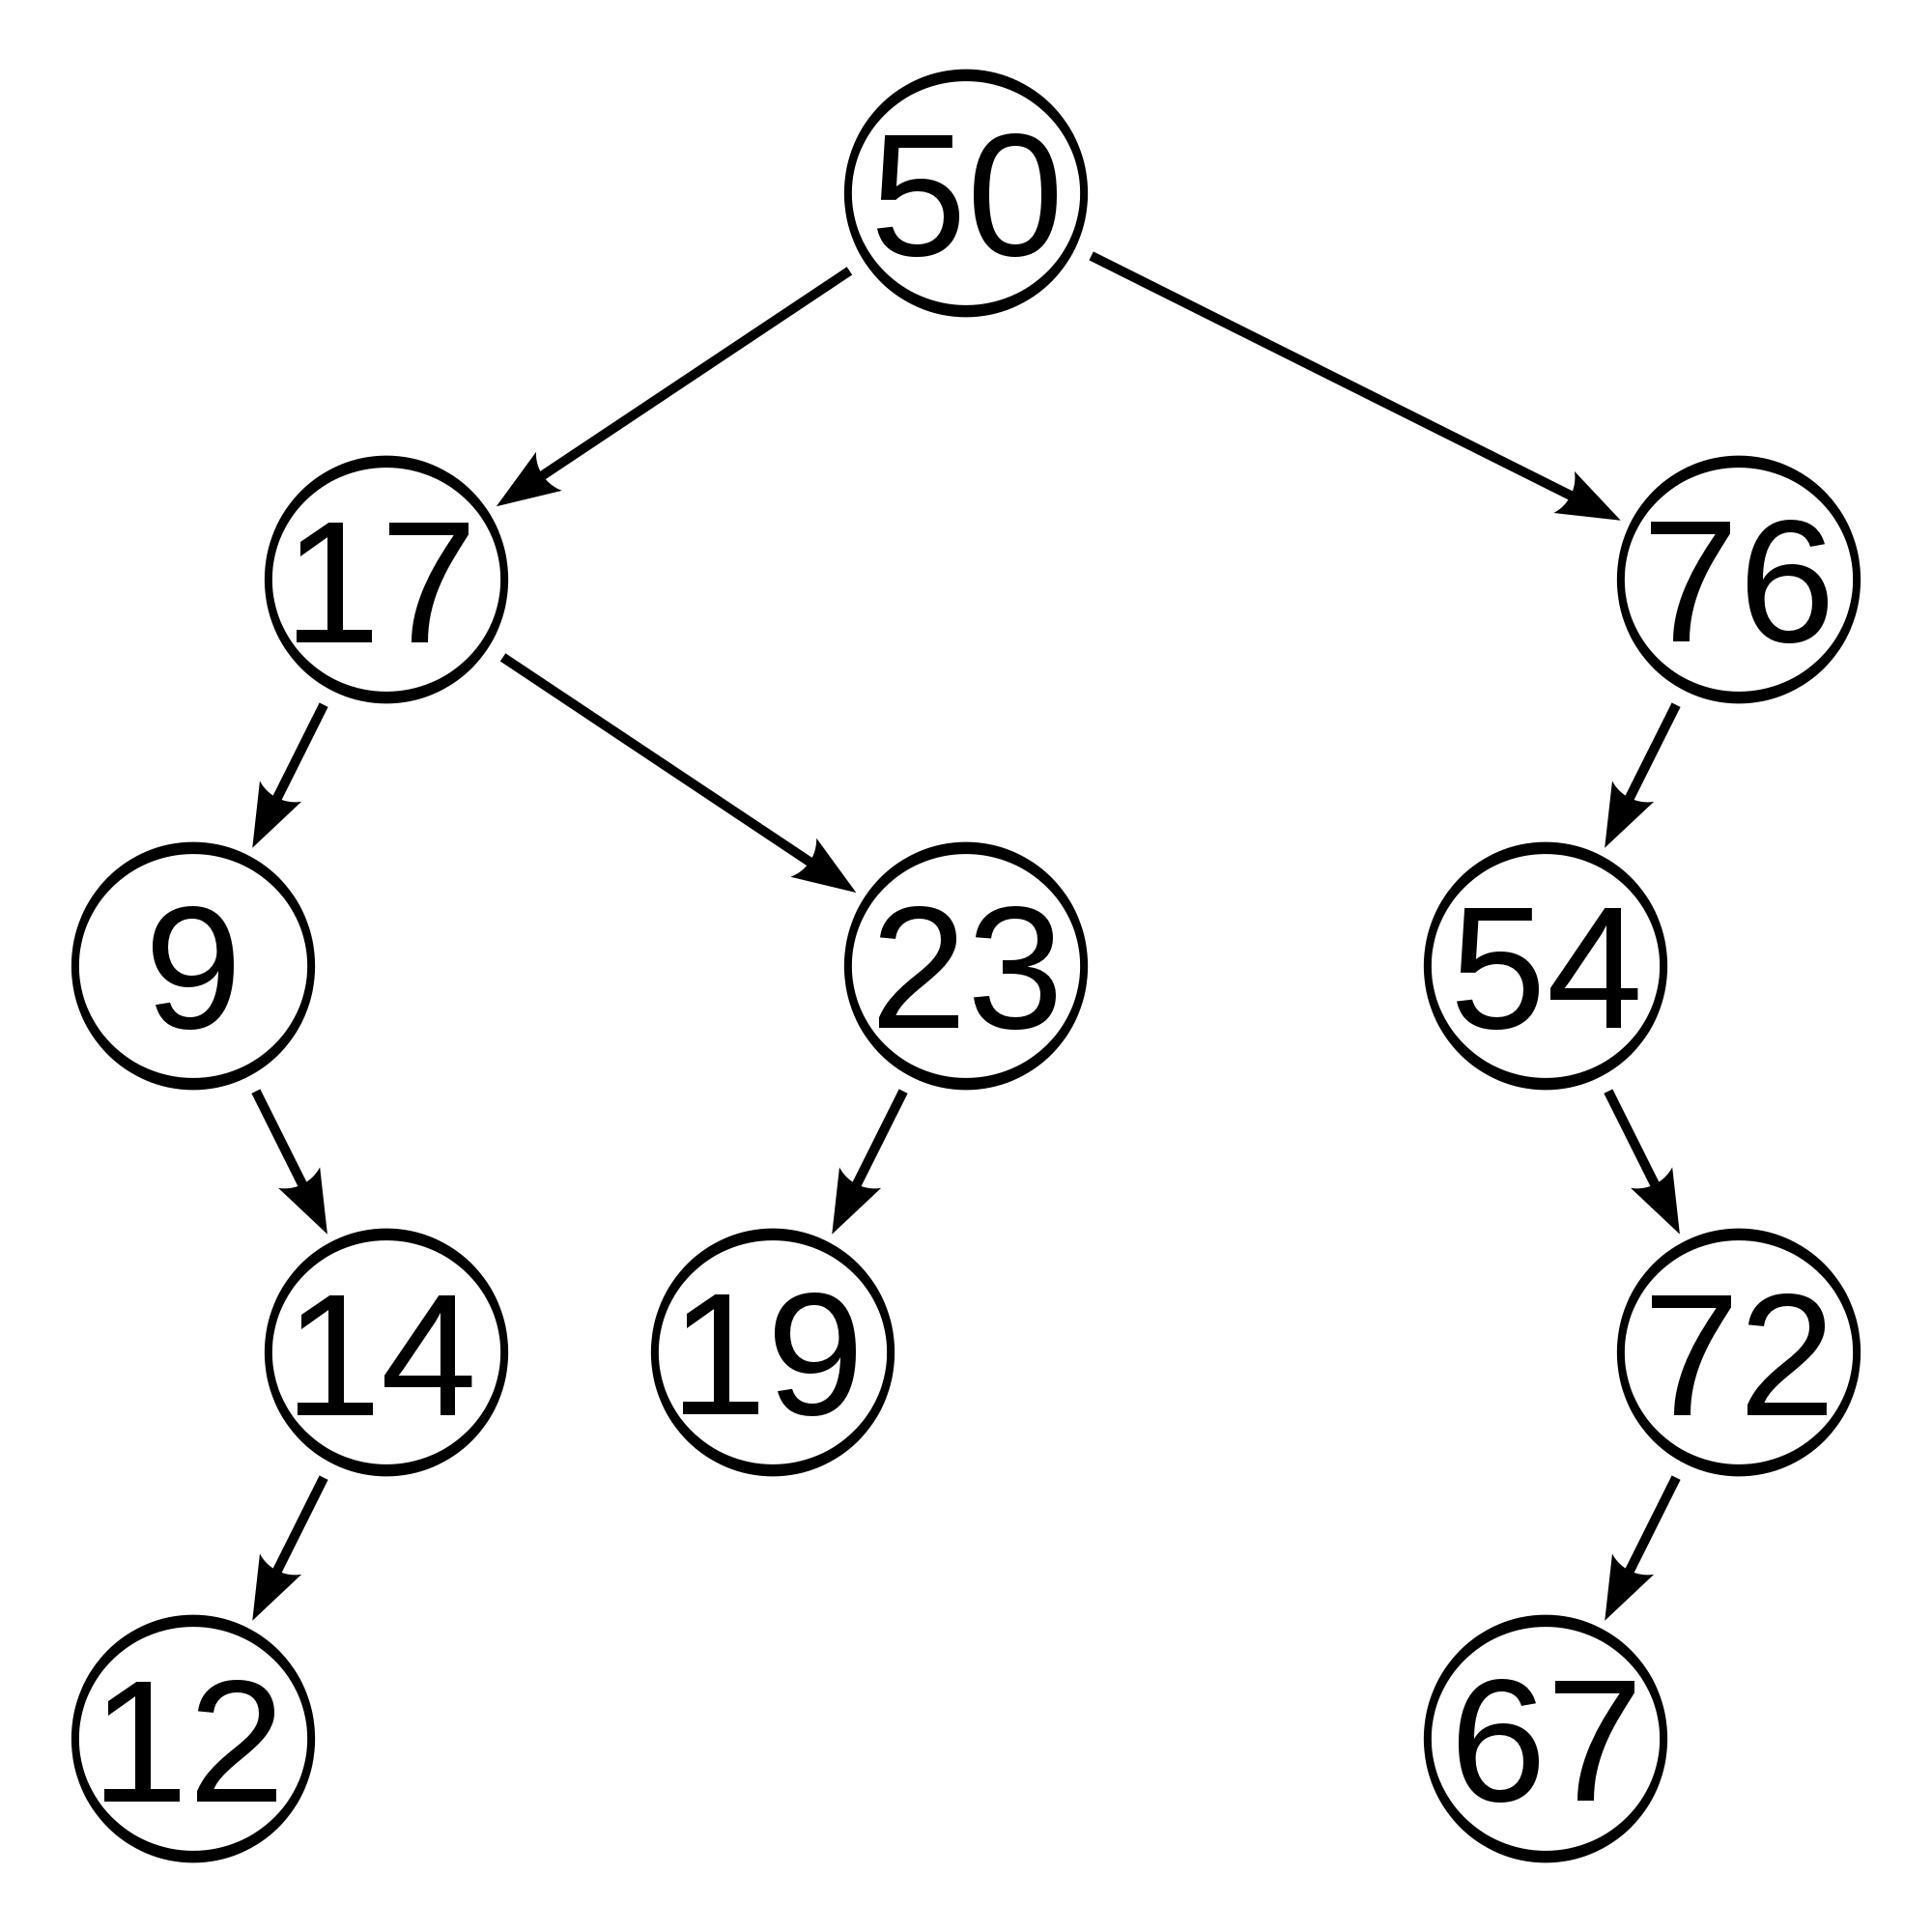
\includegraphics[scale=0.1]{../images/tree_unbl}
		\caption{Binary search tree}
	\end{figure}

It's important to notice the difference between the binary search property and the heap property. The heap property states that for each nodes, the key of the children  of a node $x$ have to be lesser the $x.key$ (both of them). The minimum element is then the root of the tree. Min heap property is less string, and hence easier to mantain, but makes the heap less poweful than the binary search tree. For instance search in a heap costs linear time. Moreover the heap is not able to print out all the element it stores in \textbf{sorted order} in linear time. It takes $\Theta(nlogn)$ since at each min extraction the min heap needs to be restored bubbling up some nodes from the new root to the leaf (in $O(log n)$) 

It is possible to print all the element stored in a search tree in sorted order simply using the so called \textbf{in order} visit of the tree. Given a tree rooted at $x$ is first visit all the nodes of the left subtree, then prints the key of $x$, and finally prints all the nodes in the right subtree.



\begin{algorithm}
\Fn{IN-ORDER(x)}{
		\If{$x=NIL$}{
			\Return \;		
		}	
		$IN-ORDER(x.left)$\;
		$process(x.key)$\;
		$IN-ORDER(x.right)$\;
	}
\caption{In order visi of a binary (search) tree }
\end{algorithm}

Intuitively this works because  the recursion walk down the leftmost path of the tree first reaching the minimum element (which is always a leaf) then prints the that element and recurs on its right subtree if present. Again starting from this node we walk our way down to the leftmost subtree, which in other word is the smallest element among all the greater element of the element just printed out. This is the successor of the printed element! So we alway print an element and its successor.

Changing the order in which we process the node and the recursive calls will make us visit the tree in different order. There are other two ways to arrange the recursive calls and the process the node (see algorithms \ref{alg:pre} and \ref{alg:pst}). 
\begin{itemize}
\item the \textbf{pre-order} visit process the current node first and then recursively visit the left and right subtrees.
\item the \textbf{post-order} visit, as the name suggest processs the current node after processing left and right subtree.
\end{itemize}


\begin{algorithm}
\Fn{PRE-ORDER(x)}{
		\If{$x=NIL$}{
			\Return \;		
		}	
		$process(x.key)$\;
		$IN-ORDER(x.left)$\;
		$IN-ORDER(x.right)$\;
	}
\caption{Pre order visi of a binary (search) tree }\label{alg:pre}
\end{algorithm}


\begin{algorithm}
\Fn{POST-ORDER(x)}{
		\If{$x=NIL$}{
			\Return \;		
		}	
		
		$IN-ORDER(x.left)$\;
		$IN-ORDER(x.right)$\;
		$process(x.key)$\;
	}
\caption{Post order visi of a binary (search) tree }\label{alg:pst}
\end{algorithm}

What is the running time of a such visit on a tree composed of $n$ nodes?
We should start noticing that a visit at least print all the elements once so its running time canno be less than $\Omega(n)$.
Noticing that no nodes is accessed twice gives us that the running time is also $O(n)$. This allows us to conclude that the running time is in reality $\Theta(n)$.

It is important to notice that the visit can also be implemented in a non-recursive procedure. non-recursive calls can be important when the height of the tree is not garanteed to be logaritmic in the number of nodes. Infact when logaritmic the recursive stack of calls has logaritmic length which is not a problem even on tree of a million elements. If the tree ha linear height, on the other hand, this could cause a stack error.

FThe in order walk can be implemented using a stack as an auxiliary data structure that stores the nodes to be processed (taking care of not adding any $NIL$) and whenever we traverse on a $NIL$ subtree we pop from the stack (which contains a valid element), process that element and go right.

\begin{algorithm}
\Fn{IN-ORDER-ITERATIVE(x,S)}{
		$S.push(x)$\;
		$current=x$\;
		\While{$S.size() > 0$}{
			\eIf{$current \neq NIL$}{
			\If{$current.left\neq NIL$}{
					$S.push(current.left)$\;
					
				}
			$current=current.left$
			}{
				$current=S.pop()$\;
				$process(p)$\;
				\If{$current.right \neq NIL$}{
				$S.push(current.right)$\;
				}
				$current=current.right$
			}
		}
		
	}
\caption{In order iterative visit }\label{alg:pst}
\end{algorithm}

The pre-order iterative visit can be implemented using a queue instead of a stack. The root is enqueued and while the queue is not empty we extract an element from the queue and process it straight away. Then we add, if present, left (first) and right children.

\begin{algorithm}
\Fn{PRE-ORDER-ITERATIVE(x,Q)}{
		$Q.push(x)$\;
		\While{$S.size() > 0$}{
			$current=Q.dequeue()$\;
			$process(p)$\;
			\If{$current.left\neq NIL$}{
				$Q.enqueue(current.left)$\;
			}
			\If{$current.right \neq NIL$}{
				$S.push(current.right)$\;
				}
	
			}
		}
\caption{Pre order iterative visit }\label{alg:pre_iter}
\end{algorithm}


\subsection{Searching}
Searching is one of the key operation that BST allows to be performed in $O(h)$. It work by checking for each visited node if the key of that node is the key we are searching for. If yes the search is succesfull and we can return a pointer to that node. If it is not then we can only search \textbf{one} of the two children. Infact if $k$ is the key to be searched and $x$ the current node then if $k > x.key $ we can continue our search on $x$'s right subtree while if $k \leq x.key $ we can continue on its left subtree. It is clear that using this procedure we walk at each iteration of the algorithm one level down till we reach a leaf. Listing \ref{alg:searchrec} and \ref{alg:searchite} are the recursive and iterative search procedures, respectively.

\begin{algorithm}
\Fn{SEARCH-REC(x,k)}{
		\If{$x==NIL$}{
			\Return NIL\;
		}		
		\If{$x.key == k$}
		{
			\Return x\;
		}
		\If{$x.key \leq k$}
		{
			\Return SEARCH-REC($x.left,k$)\;
		}
		\Return SEARCH-REC($x.right,k$)\;
		}			
\caption{BST search recursive.}\label{alg:searchrec}
\end{algorithm}


\begin{algorithm}
\Fn{SEARCH-ITE(root,k)}{
		\While{$root \neq NIL \wedge root.key \neq k$}{
				\If{$root.ket \leq k$}{
					$root=root.left$\;
				}\Else{
					$root=root.right$\;
				}
			}
			\Return $root$;		
		}			
\caption{BST search iterative.}\label{alg:searchite}
\end{algorithm}


\subsection{Minimum and Maximum}
Minimum and maximum are other two operation supported by BST in $O(n)$ time.
Minimum is the element which is smaller than any other element in the structure. Given a node, from the BST property we already know that all the element smaller than it are in its left subtree.
The minimum element is then the leftmost node not having any left child. This translates to: this node has no element smaller than it.
On the other hand the same line of reasoning holds for the \textit{maximum} element. It is the rightmost node not having right child. Listings \ref{alg:minimum} and \ref{alg:maximum} are the procedures for extracting the minimum and the maximum element from a treee rooted at $root$ (assume not to be $NIL$).

\begin{algorithm}
\Fn{MINIMUM(root)}{
		\While{$root.left \neq NIL$}{
					$root=root.left$\;
			}		
			\Return $root$;
		}			
\caption{BST search iterative.}\label{alg:minimum}
\end{algorithm}

\begin{algorithm}
\Fn{MAXIMUM(root)}{
		\While{$root.right \neq NIL$}{
					$root=root.right$\;
			}		
			\Return $root$;
		}			
\caption{BST search iterative.}\label{alg:minimum}
\end{algorithm}

\subsection{Predecessor and Successor}
Successor and predecessor of a node $x$ are defined as the nodes whose key is the next greater and smaller than $x.key$.
By the BST property then it follows that the successor is the element which lies in the right subtree of $x$ (since it is greater). Among all the greater elmenets we should take the smallest one (i.e. the minimum among them). So the successor element is the minimum of the right subtree of $x$. What if the right subtree for $x$ does not exists? The successor must be somewhere in the upper levels,a nd more specifically it must be the first ancestor $x_a$ of $x$ for which $x$ is in \textbf{not} $x_a$'s right subtree( See Figure \ref{fig:bst_successor}). Being in the right subtree of a node $n$ means that out key is greater than the key $n$ (how can a node which its key is smaller than ours be our successor? Its impossible, that is why we look for the first ancestor for which we are in its left subtree, because our key is smaller than its key).
Take for instance the node with key $7$ in figure \ref{fig:bst_successor}. Its successor is node $8$ because if we keep seeking parents points from $7$ at some point we arrive at the point in which the current node is not the right child of a node.

Again fot the simmetry of the BST property the predecessor is the maximum among all the smaller or equal element of $x$. 
Listings \ref{alg:succesor} and \ref{alg:predecessor} are the procedures for extracting the successor and predecessor elements.

	\begin{figure}
	\label{fig:bst_successor}
	\centering
		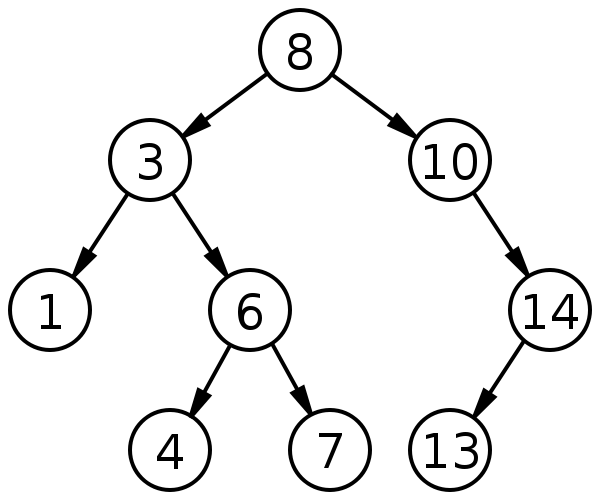
\includegraphics[scale=0.5]{../images/bst_successor}
		\caption{Binary search tree successor and predecessor.}
	\end{figure}
\begin{algorithm}
\Fn{SUCCESSOR(x)}{
		\If{$x \neq NIL \wedge x.right \neq NIL$}{
			\Return $MINIMUM(x.right)$\;
		}
		\While{$p \neq NIL \wedge p.right = x  $}
		{
			$x=p$\;
			$p=x.parent$\;
		}
		\Return $p$\;
		}			
\caption{BST successor procedure.}\label{alg:successor}
\end{algorithm}

\begin{algorithm}
\Fn{PREDECESSOR(x)}{
		\If{$x \neq NIL \wedge x.left \neq NIL$}{
			\Return $MAXIMUM(x.left)$\;
		}
		$p=x.parent$
		\While{$p \neq NIL \wedge p.left = x  $}
		{
			$x=p$\;
			$p=x.parent$\;
		}
		\Return $p$\;
		}			
\caption{BST predecessor procedure.}\label{alg:successor}
\end{algorithm}

\subsection{Insert and Delete}

Insertion and delete are two operation that modifiy the structure of the tree. We should take care of performing them ensuring that the BST property hold at the end of each of these two operation execution on the tree. BST has to be and invariant of these procedures.
As we will see insertion is quite easy to design and implement while the delete operation requires some extra care.
\subsubsection{Insert}
The insertion procedure solves the following problem: given a key $k$ we would like to insert it into the tree rooted at $root$. 
The idea is that we need to search for the right spot where to insert  a newly constructed element which keys is $k$. 
The procedure shown in Listing \ref{alg:insert} outline the ided behind insertion in a BST (See Figure \ref{fig:insertion}).
\begin{algorithm}
\Fn{INSERT(root,z)}{
			\If{$root==NIL$}{
				$root=z$\;
				\Return \;			
			}
			$y=root$\;
			\While{$y \neq NIL$}{
				\If{$y.key \geq z.key$}{$y=y.left$\;}
				\If{$y.key < z.key$}{$y=y.right$\;}
			}
			$z.parent=y$\;
			\If{$y.key \geq z.key$}{$y.left=z$\;}
			\Else{$y.right=z$\;}
			
}
\caption{Iterative BST insert procedure.}\label{alg:insert}
\end{algorithm}

\begin{figure}
	\label{fig:insertion}
	\centering
		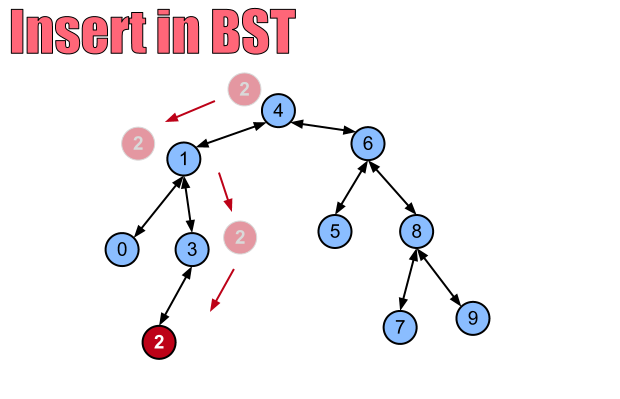
\includegraphics[scale=0.7]{../images/bstinsert}
		\caption{Inserting a node with key $2$ in a BST.}
	\end{figure}

We navigate the BST from the root to the leafs and we stop as soon we found a $NIL$ spot which is good for inserting the element $z$ (good means that preserves the BST property).
Let's call this element $y$. We need to set $z$'s parent pointer to $y$ and make $z$ child of $y$ by updating the correcnt $y$ child pointer.

\begin{algorithm}
\Fn{INSERT(root,c,p,z)}{
			\If{$p == NIL$}{
				$root=z$\;
				\Return \;
			}
			$side=NIL$\;	
			\If{$c == NIL$}{
				$z.p=p$\;
				
			\If{$z.key \leq p.key$}{				
				$p.left=z$\;
			}\Else{
				$p.right=z$\;			
			}
			
			}\Else{
				\If{$z.key \leq p.key$}{				
				$INSERT(root,c.left,c)$\;
			}\Else{
				$INSERT(root,c.right,c)$\;
			}
			}
			
	}
\caption{Recursive BST insert procedure.}\label{alg:insert}
\end{algorithm}


\subsubsection{Delete}
Delete operation is a bit more delicate and requires some extra care. Let's note that deleting a node with no children at all is an easy case since it is a leaf. Deleting a leaf does not ruin the BST property.
For instance take the node $13$ in figure \ref{fig:bst_successor}. Deleting it leaves the tree withouth doing any further operations preserves the BST property. Another easy case is when the node has only one child (the node $10$ or $14$ in figurer \ref{fig:bst_successor} for instance).  What we need to do is to delete that node and move the only one substree (right or left, in its entirety) up one level to the just deleted node parent node. 
Let's say for instance that we are about to delete node $10$. What we have to do is to set $8$'s right child pointer to node $14$ and to update $14$'s parent pointer such it points to node $8$. In other words we elevate the only present child   to the position of the to be deleted node ($z$) by modifying $z$'parent ($8$  in this case).

If $z$ has both children then we can't simply delete the node because this would leave an hole in the data structure, and consequently, some nodes would be unreachable. For instance imagine we are about to delete node number $6$ in Figure \ref{fig:bst_successor}. Deleting that node would leave nodes $4$ and $7$ unlinked and unreachable from the root!
We need to substitute $z=6$ with some other node. Which one? The only node which can be substituted to $z$ and still satisfies the BST is $z$ successor because all nodes at $z$'s left subtree would still be lesser or equal than $z$'s successor and all element on $z$'s right subtree would be still greater than $z$ successor (which will not belong to $z$ subtree any more and was smaller than all element in $z$ right subtree, being the minimum among them!).
If $z's$ successor ($y$) is $z$'s right child then we simply substitute $z$ by $y$. 
If is not then we need to make $y$ right subtree (the only one present since it's $z$'s  successor) left child of $y$ parent (which cannot be  $z$!) and then move $y$ in place of $z$.


As and example take the node $6$ in Figure \ref{fig:insertion}. If we substitute $6$ by $7$, its successor, then the BST property is still satisfied since $5$ is still less than $7$ and $8$ and $9$ are greater than $7$.

\begin{figure}
	\label{fig:insertion}
	\centering
		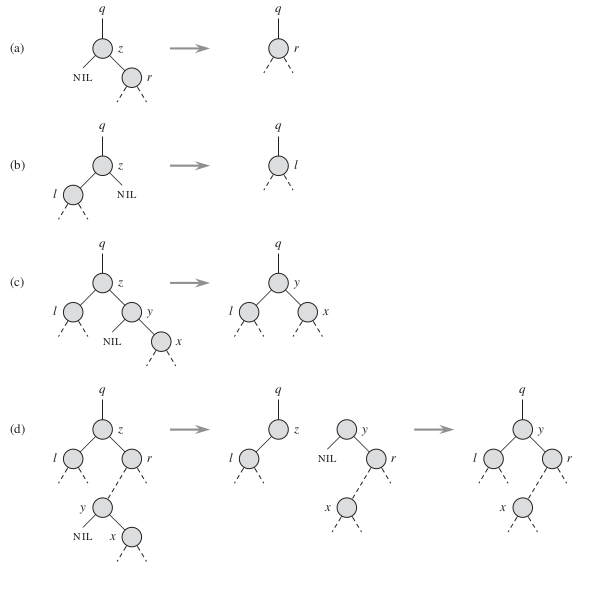
\includegraphics[scale=0.7]{../images/bstdelete}
\caption{Deleting a node $z$ from a BST. case \textbf{(a)} deals with the case $z$ has not left child. Its right child (which may be NIL, and if it is, this handle the case where both children are NIL) is substituted to $z$. Case \textbf{(b)} is when $z$ has only left subtree, in this case again we simply substitute $z$ by $z$'s left child. Case \textbf{(c)} is when $z$ has both children  but is successor is $z$ right child! In this case we simply elevate $y$ at $z$ place without modifying the structures of any node at lower levels. Case \textbf{(d)} deals with the case when $z$ successor is not $z$'s right child. 
If this is the case then we can't simply move $y$ in place of $z$ since $y$ may carries a whole subtree (right one) with it. We need to move $y$ right subtree in place of $y$ first and then safely move $y$ in place of $z$. }
	\end{figure}

Since we are moving subtree around it is useful to write a utility procedure that takes a tree and two subtree rooted at $u$ and $v$ respectively. Goal of this procedure is to substitute $u$ with $v$ making sure that parent links are correctly set.

\begin{algorithm}
\Fn{TRANSPLANT(root,u,v)}{
			\If{$u==NIL$}{
				$root=v$\;
				\Return \;			
			}
			\If{$u.p.left==u$}{
				$u.p.left=v$\;
			}\Else			
			{
				$u.p.right=v$\;
			}
			\If{$v \neq NIL$}{
				$v.p = u.p$\;			
			}
}
\caption{TRANSPLANT procedure. It takes two subtree rooted at $u$ and $v$ and substitue $u$ with $v$ making sure that parent links are preserved.}\label{alg:transpant}
\end{algorithm}

Using precedure \ref{alg:transpant} it is not hard to write a procedure for deleting a node into a BST.
\begin{algorithm}
\Fn{DELETE(root,z)}{
			\If{$Z.left==NIL$}{
				$TRANSPLANT(root,z,z,right)$\;
				\Return \;			
			}
			\If{$Z.right==NIL$}{
				$TRANSPLANT(root,z,z,left)$\;
				\Return \;
			}
			$y=SUCCESSOR(root,z)$\;
			\If{$y \neq z.right$}{
					$TRANSPLANT(root, y, y.right)$\;
					$y.right=z.right$\;
					$y.right.p=y$\;
			}
			$TRANSPLANT(root,z,y)$\;
			$y.left=z.left$\;
			$y.left.p=y$\;
			
		
}
\caption{Delete procedure. The four possible cases are handled.  Note in particlar how the case where $z$ has both children is handled. We first find its successor $y$ (node with the  smallest in its (NOT NIL) right subtree. Since we want to move $y$ from its original location and put in place of $z$. Now if $y$ is $z$'s right child then we first move $y$ right subtree in plce of $y$. We do so by updating $y$'s parent (inside transplant procedure) and updating $x$ parent pointer  to points to $y$ parent $r$. We subsequentially change $y$ right child pointer to point to $z$ right child. We can safely move $y$ into place of $z$. We do so by transplanting $y$ into $z$We do so updating $z$'s parent pointer (inside transpant operation) and then updating $z$ left child to point to its new parent $y$.}\label{alg:transpant}
\end{algorithm}

Complexity of DELETE procedure is linear in the height of the tree. All operations performed are constant time but successor which is $O(h)$.

\section{Self Balancing Tree}
\subsection{B Tree}
\subsection{B+ Tree}

\subsection{Adelson-Velsky Landis Tree - AVL Tree}
\subsection{Red Black Tree}
\subsection{Splay Tree}


\section{Space-partitioning trees}
\subsection{Kd Tree}
\subsection{R Tree}